\documentclass[a4paper,12pt]{article}

\usepackage{../usfdvl}


\title{Worksheet 8}
\SetDocumentFooter{}{}


\begin{document}

\maketitle

\worksheetGroundRules


\vspace{5pt}
\section{Assignment}

\begin{itemize}



\item For the following point set, find perform spatial subdivision using a: grid; quadtree; and kd-tree. Show the algorithm using the following pages. Be sure to show all of the steps and the order of steps for the algorithm (show both the division and resulting tree).

\begin{center}
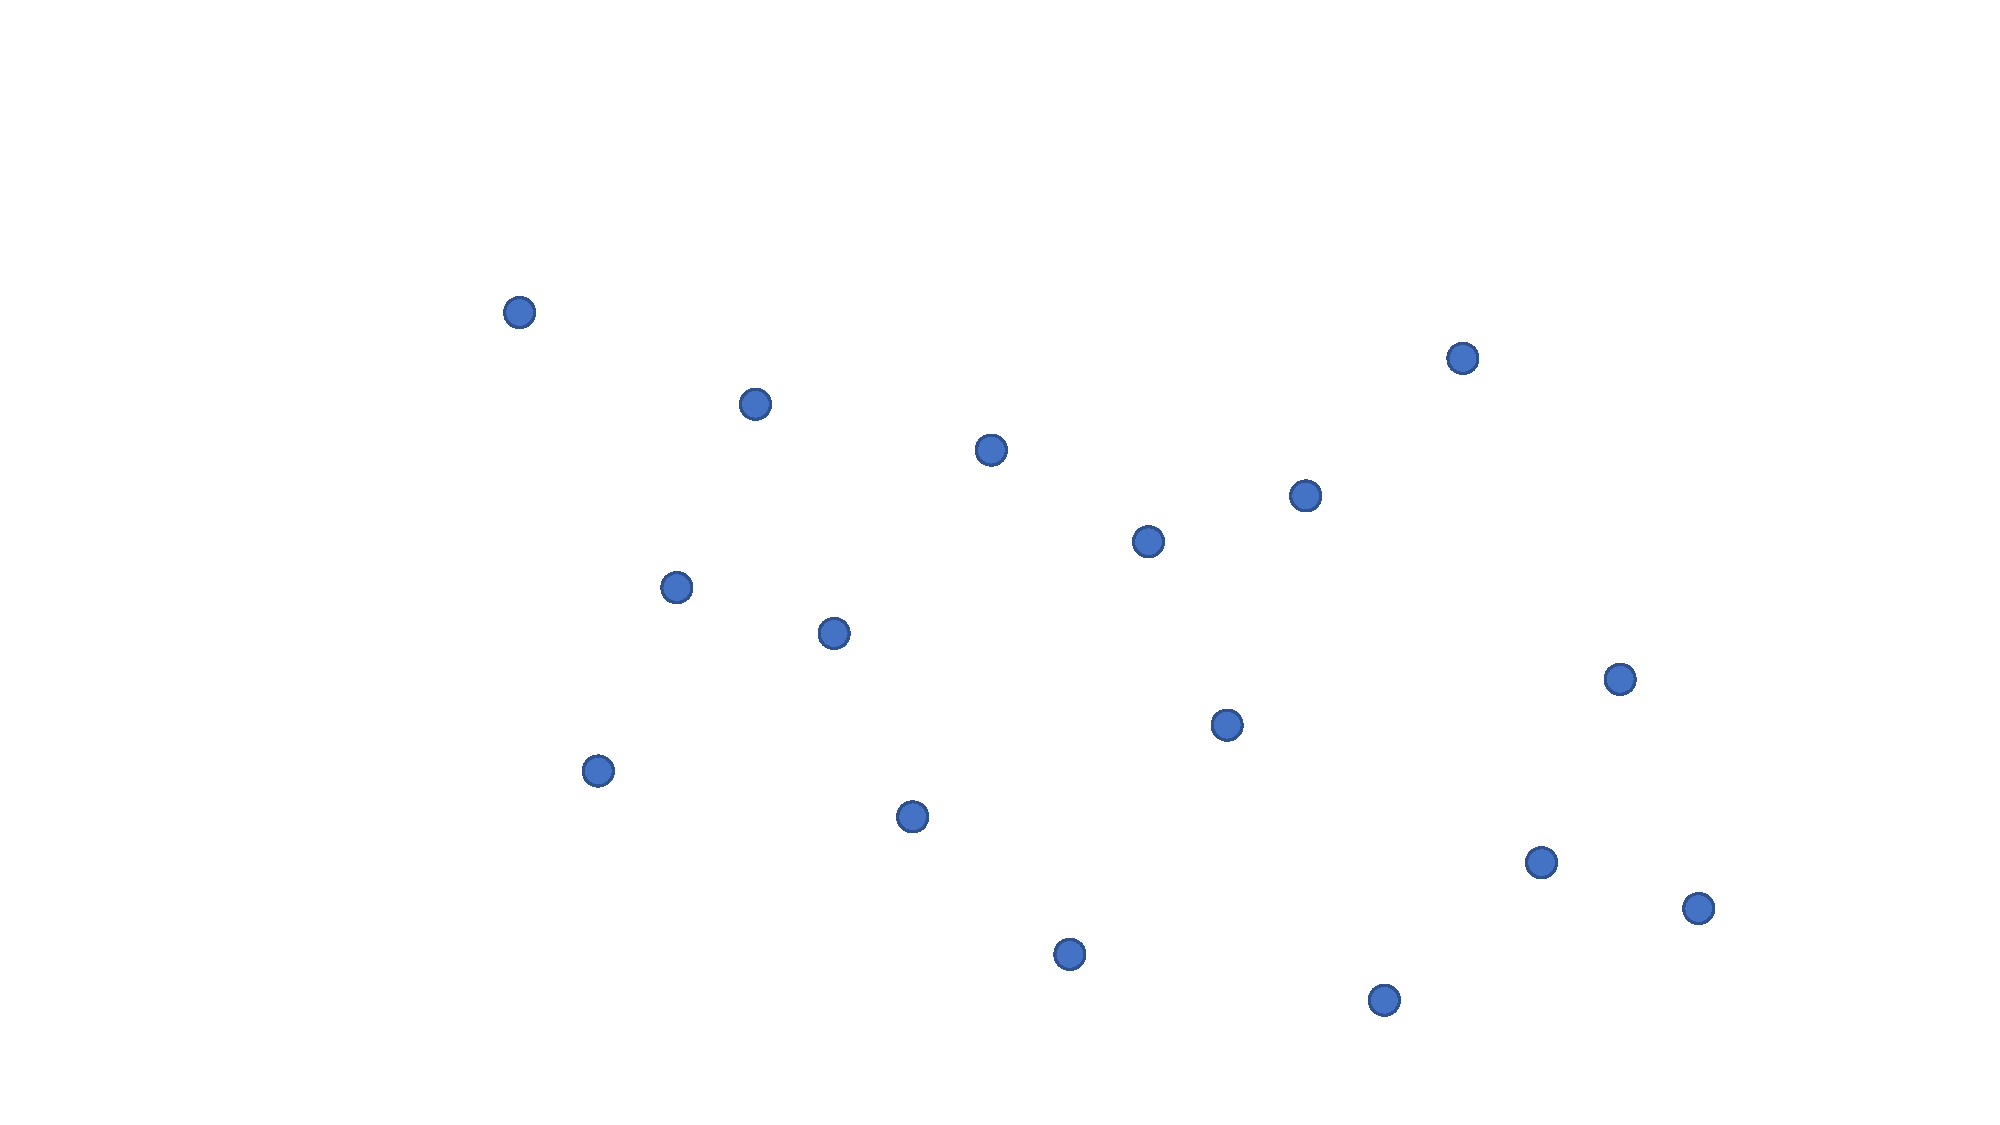
\includegraphics[width=9.5cm]{../images/spatial_subd.pdf}
\end{center}


\item For each algorithm, determine some example point sets which produce best and worst case spatial subdivision and query time.


\end{itemize}


\worksheetSubmission




\newpage

\begin{center}
\begin{tabular}{|c|c|}
\hline
 & \\
\hspace{10pt}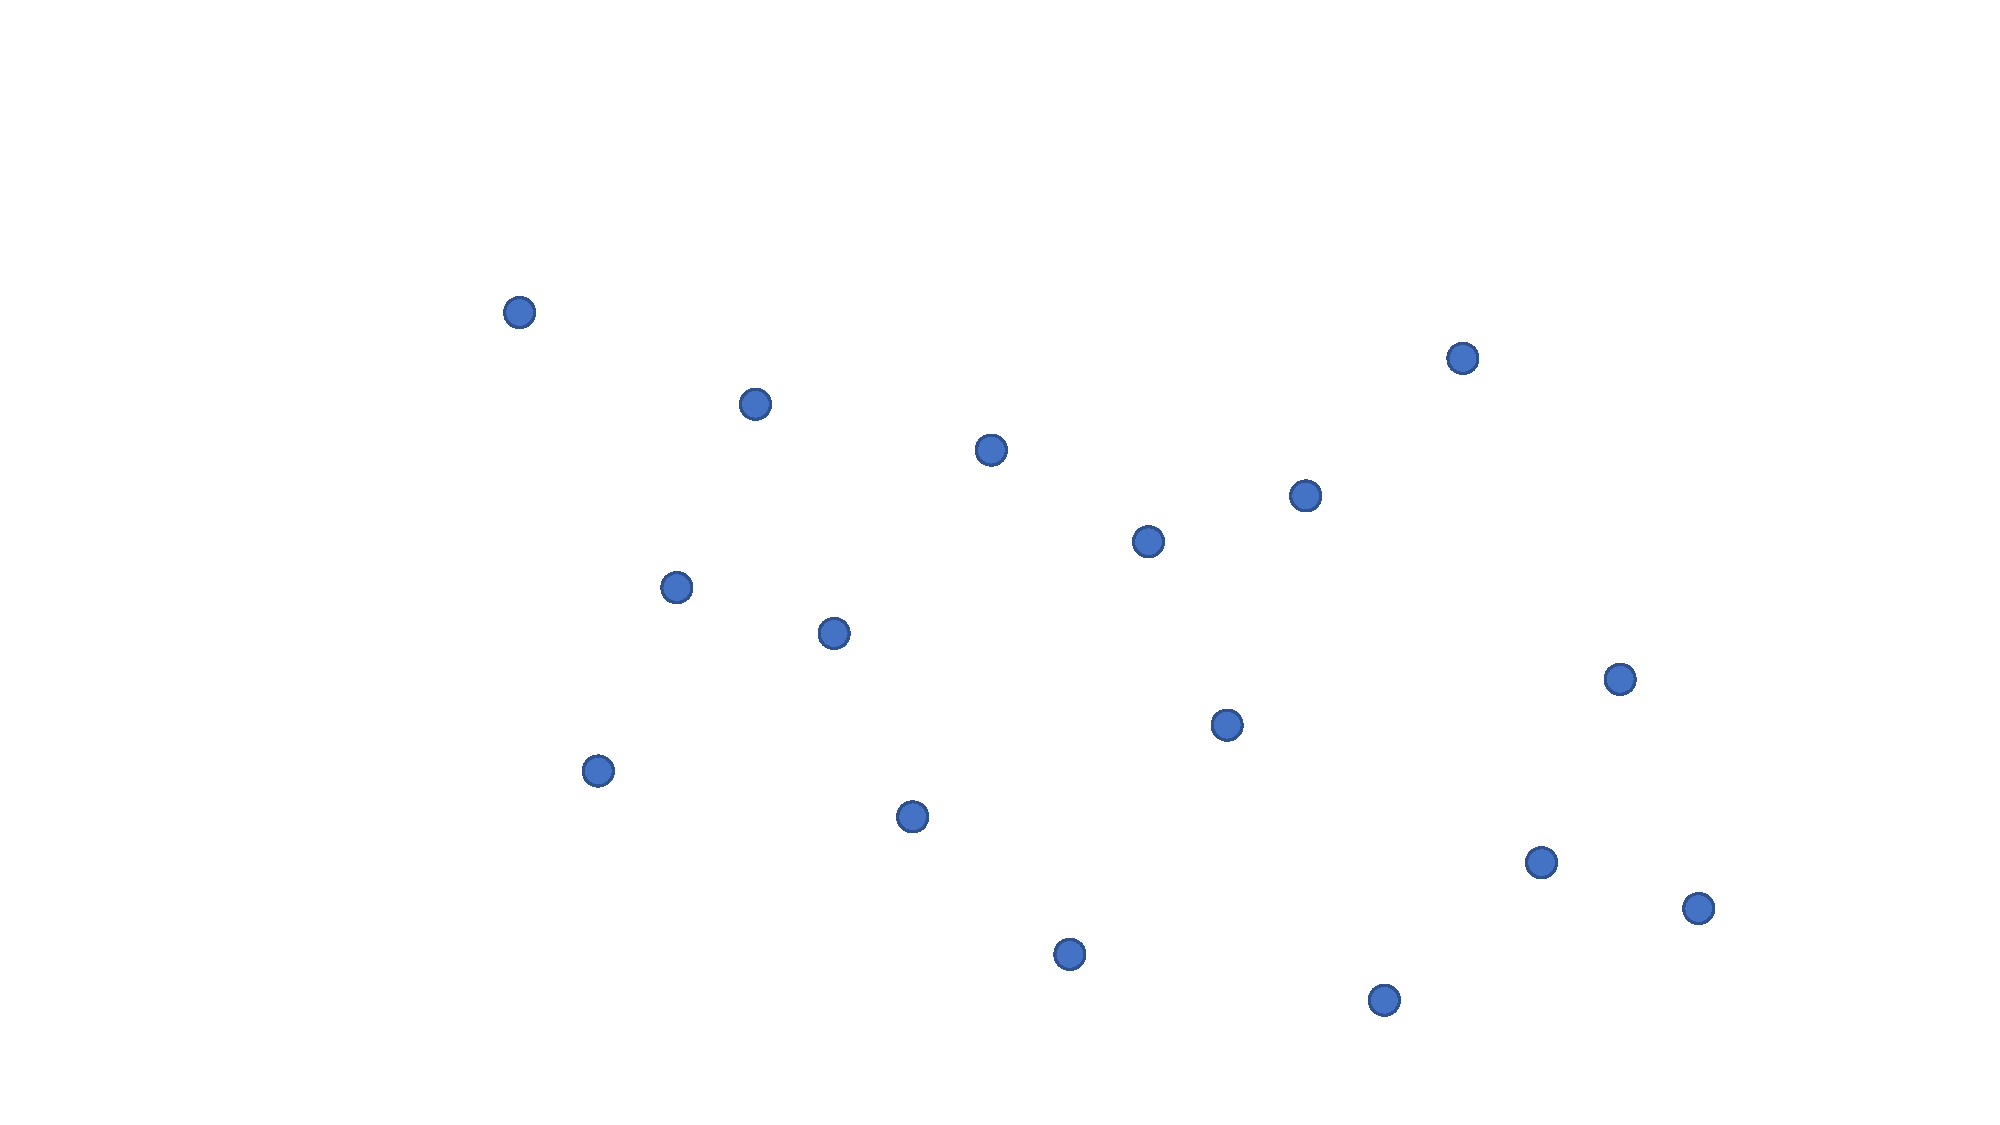
\includegraphics[width=7.5cm]{../images/spatial_subd.pdf}
\hspace{10pt} & \hspace{175pt} \\
 & \\
\hline
 & \\
\hspace{10pt}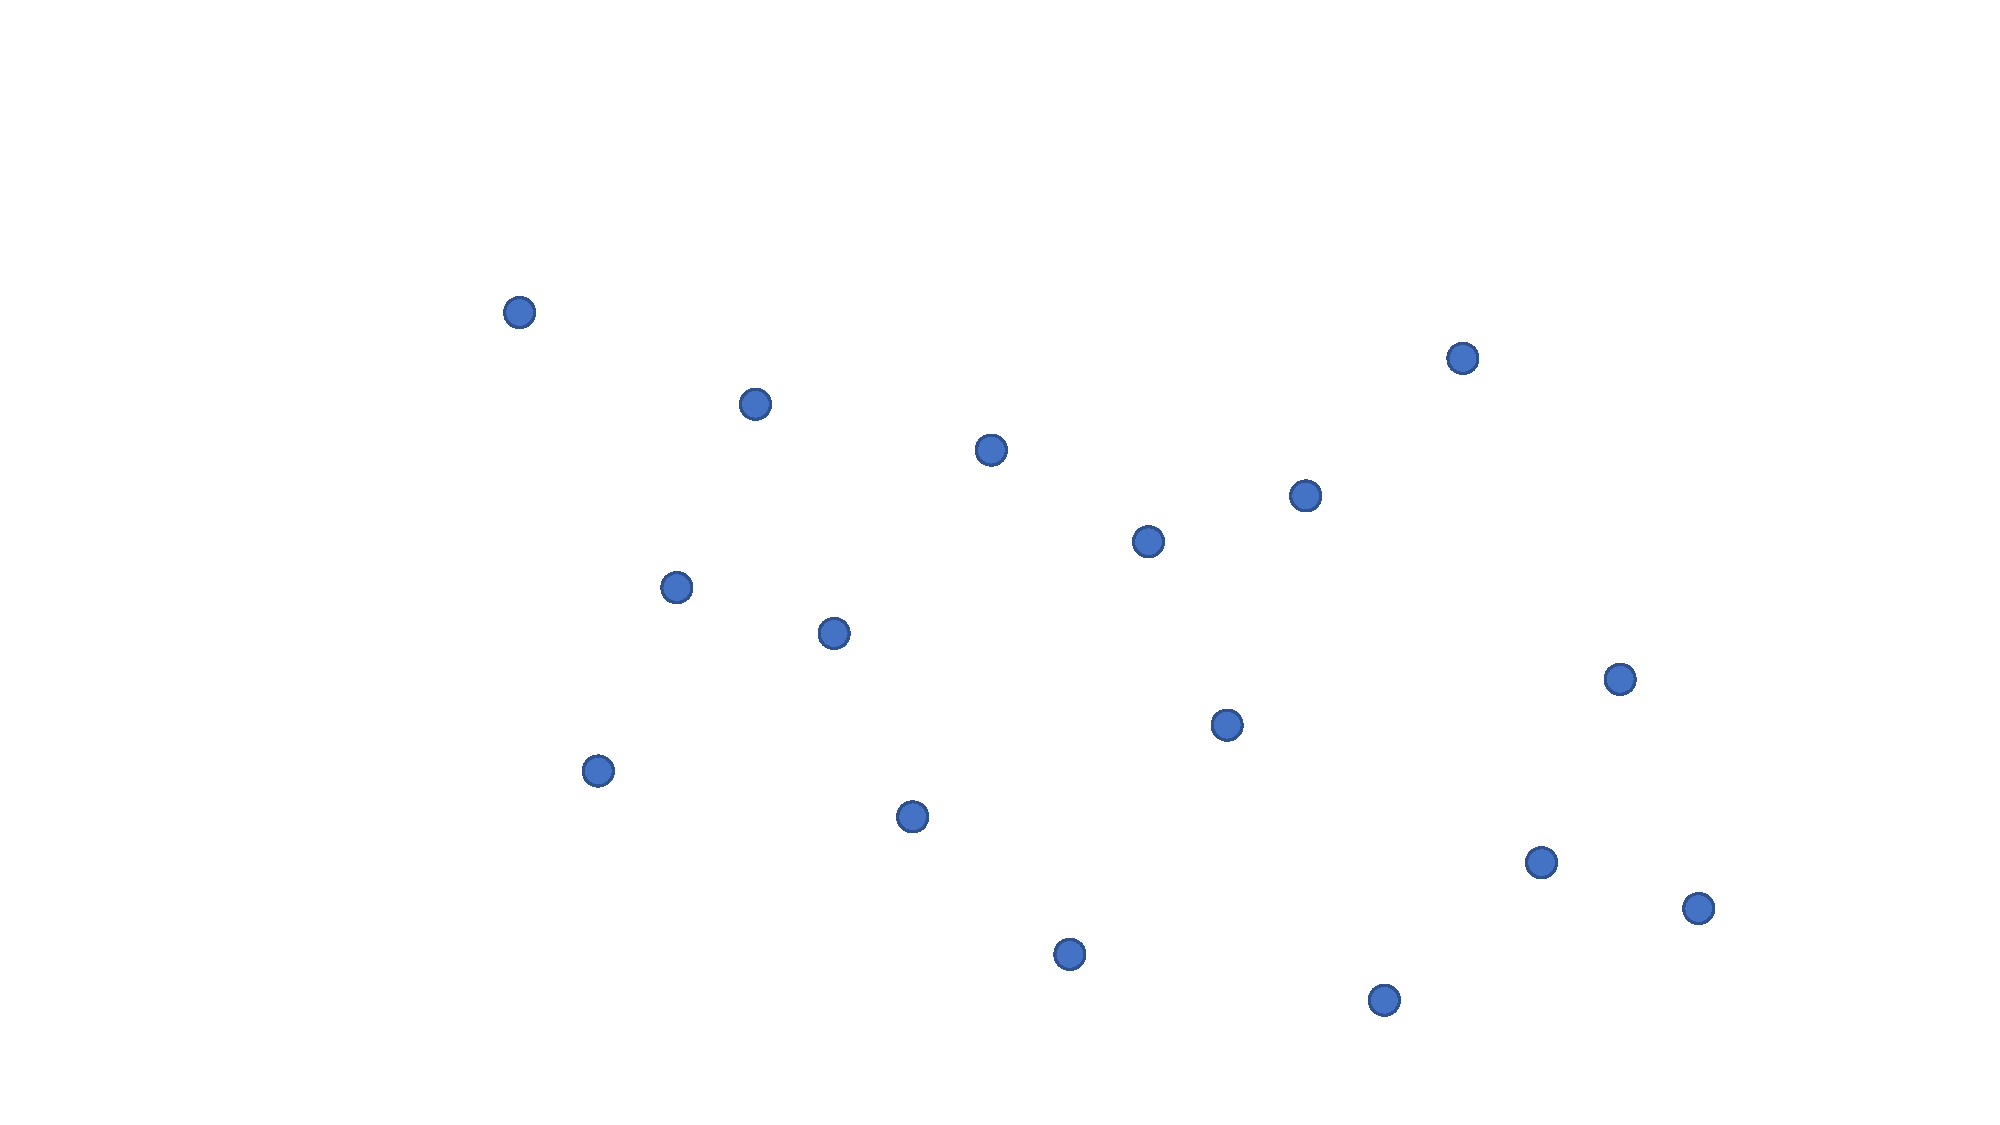
\includegraphics[width=7.5cm]{../images/spatial_subd.pdf}
\hspace{10pt} & \hspace{10pt} \\
 & \\
\hline
 & \\
\hspace{10pt}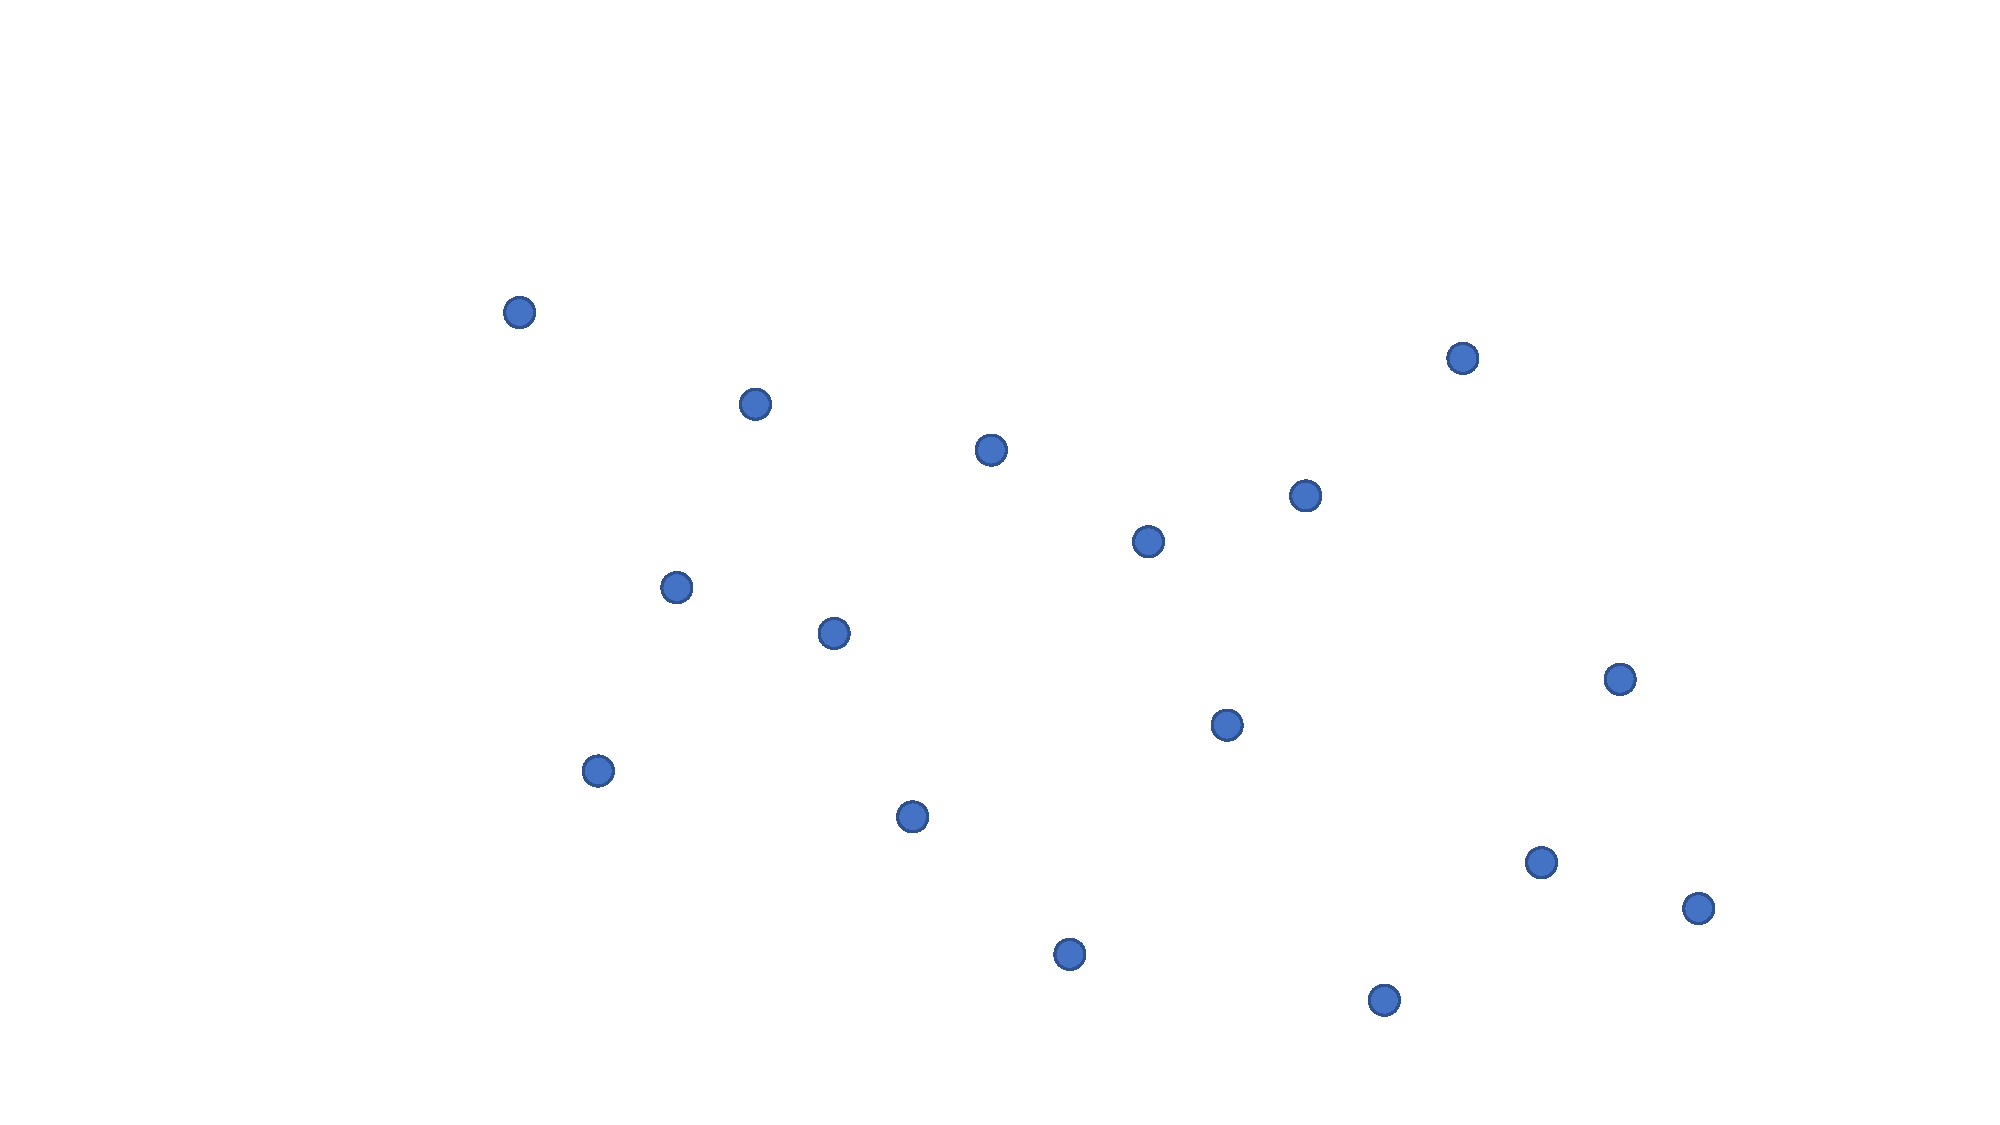
\includegraphics[width=7.5cm]{../images/spatial_subd.pdf}
\hspace{10pt} & \hspace{10pt} \\
 & \\
\hline
 & \\
\hspace{10pt}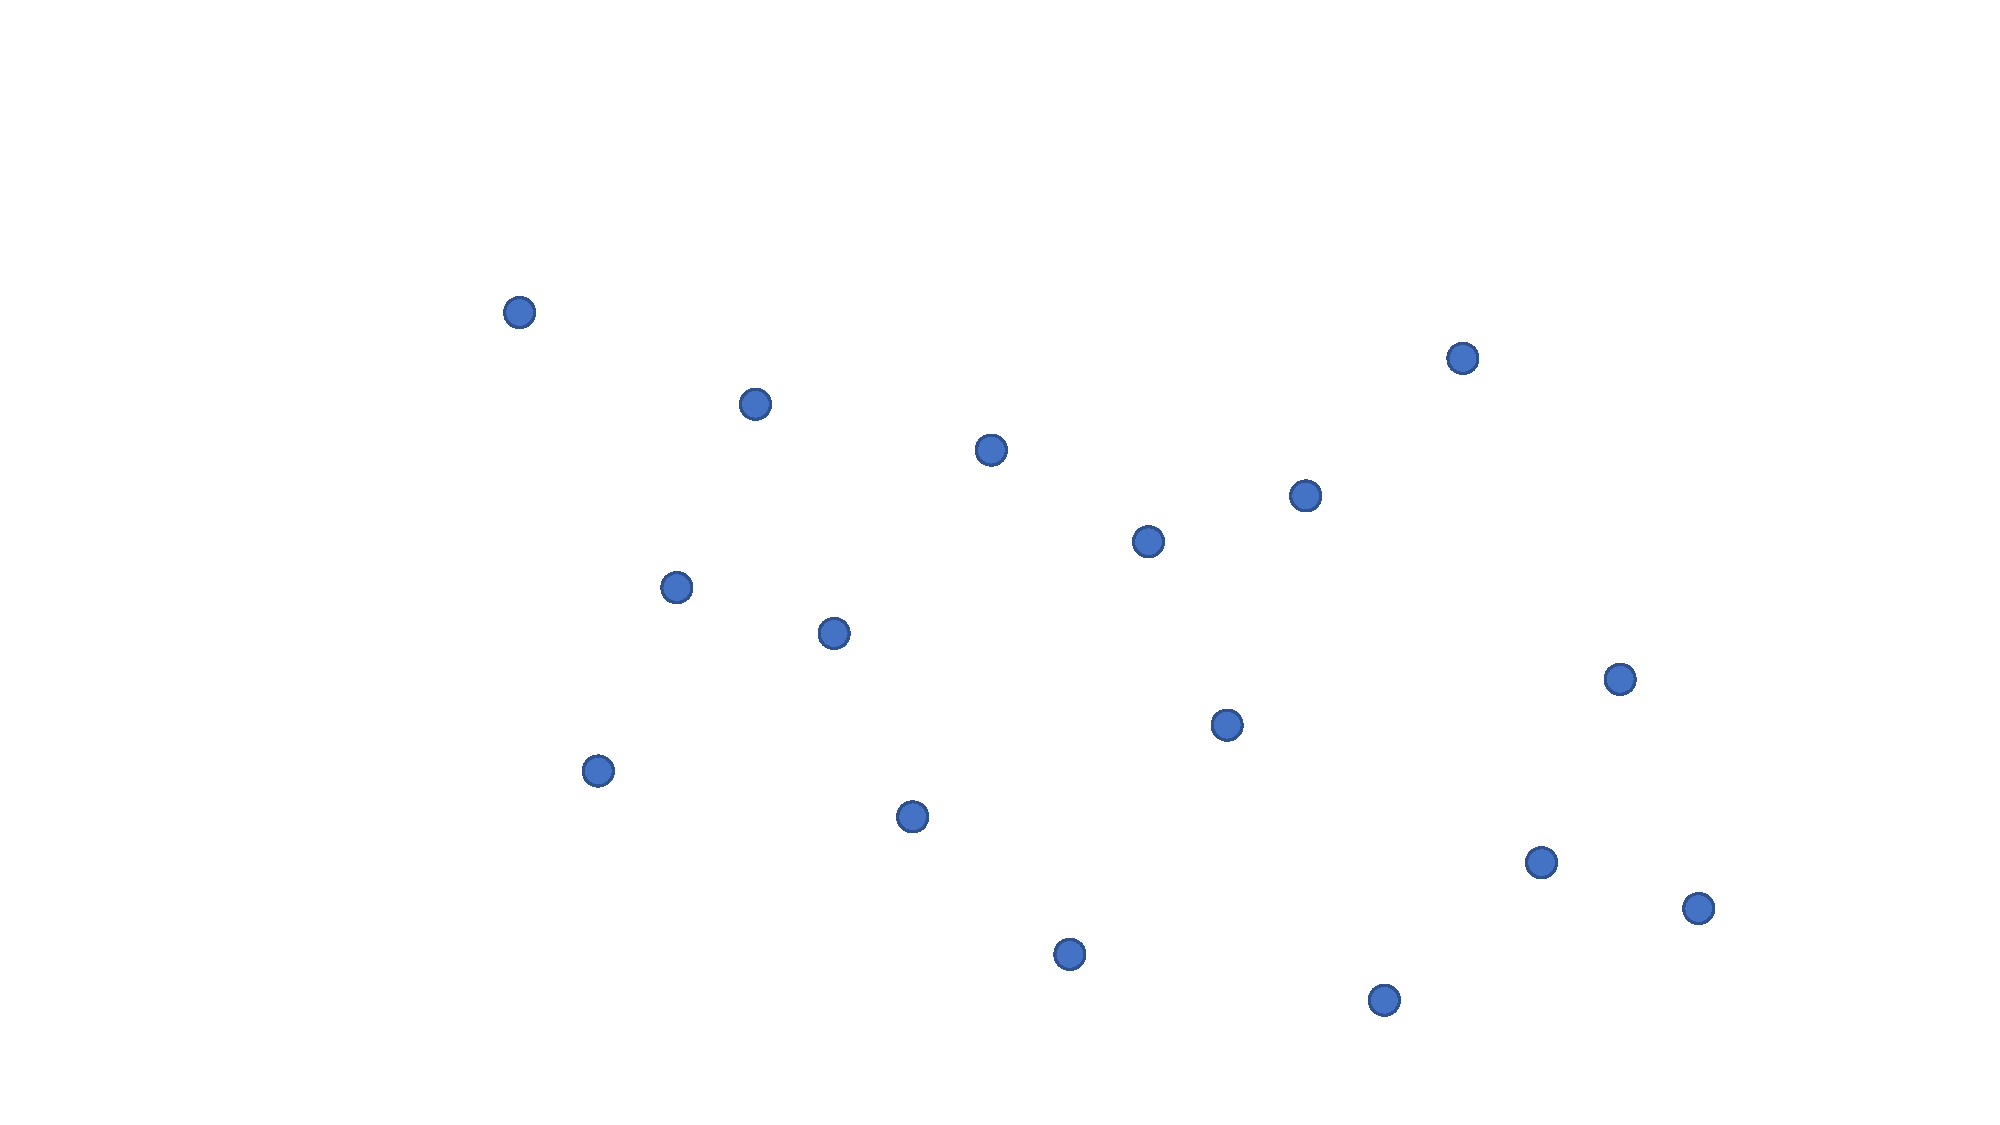
\includegraphics[width=7.5cm]{../images/spatial_subd.pdf}
\hspace{10pt} & \hspace{10pt} \\
 & \\
\hline
\end{tabular}
\end{center}


\end{document}



